\documentclass{article}
\usepackage{fancyhdr}
\usepackage{graphicx}
\pagestyle{fancy}
\usepackage{geometry}
\usepackage{listings}
\usepackage{longtable}
\usepackage{enumitem}
\usepackage{color}
\usepackage{fontspec}
\geometry{a4paper, scale=0.75}
\lhead{Yangzhe Xie}
\chead{SWEN90006: Assignment 1}
\rhead{1029787}
\renewcommand{\headrulewidth}{0.4pt}
\renewcommand{\headwidth}{\textwidth}
\definecolor{keywordcolor}{rgb}{0.8,0.1,0.5}
\definecolor{webgreen}{rgb}{0,.5,0}
\definecolor{bgcolor}{rgb}{0.92,0.92,0.92}
\lstset{language=[AspectJ]Java,
    %backgroundcolor=\color{bgcolor}, 设置背景色
    basicstyle=\small,
    commentstyle=\color{blue} \textit, 
    showstringspaces=false,
    captionpos=b,
    xleftmargin=2em,
    xrightmargin=2em, 
    aboveskip=1em
    %numbers=left,
    %numberstyle=\small
}

\title{SWEN90006: Assignment 1}
\author{Name: Yangzhe Xie\\Student number: 1029787\\Email: yangzhe.xie@student.unimelb.edu.au}

\date{\today}
\begin{document}

\maketitle
\thispagestyle{fancy}

\section{Task 1}
\subsection{Test template trees}
Figure 1 - 4 shows the test template trees for the API addUser, loginUser, updateDetails, and retrieveDetails respectively.
\begin{figure}[hbt!]        
\center{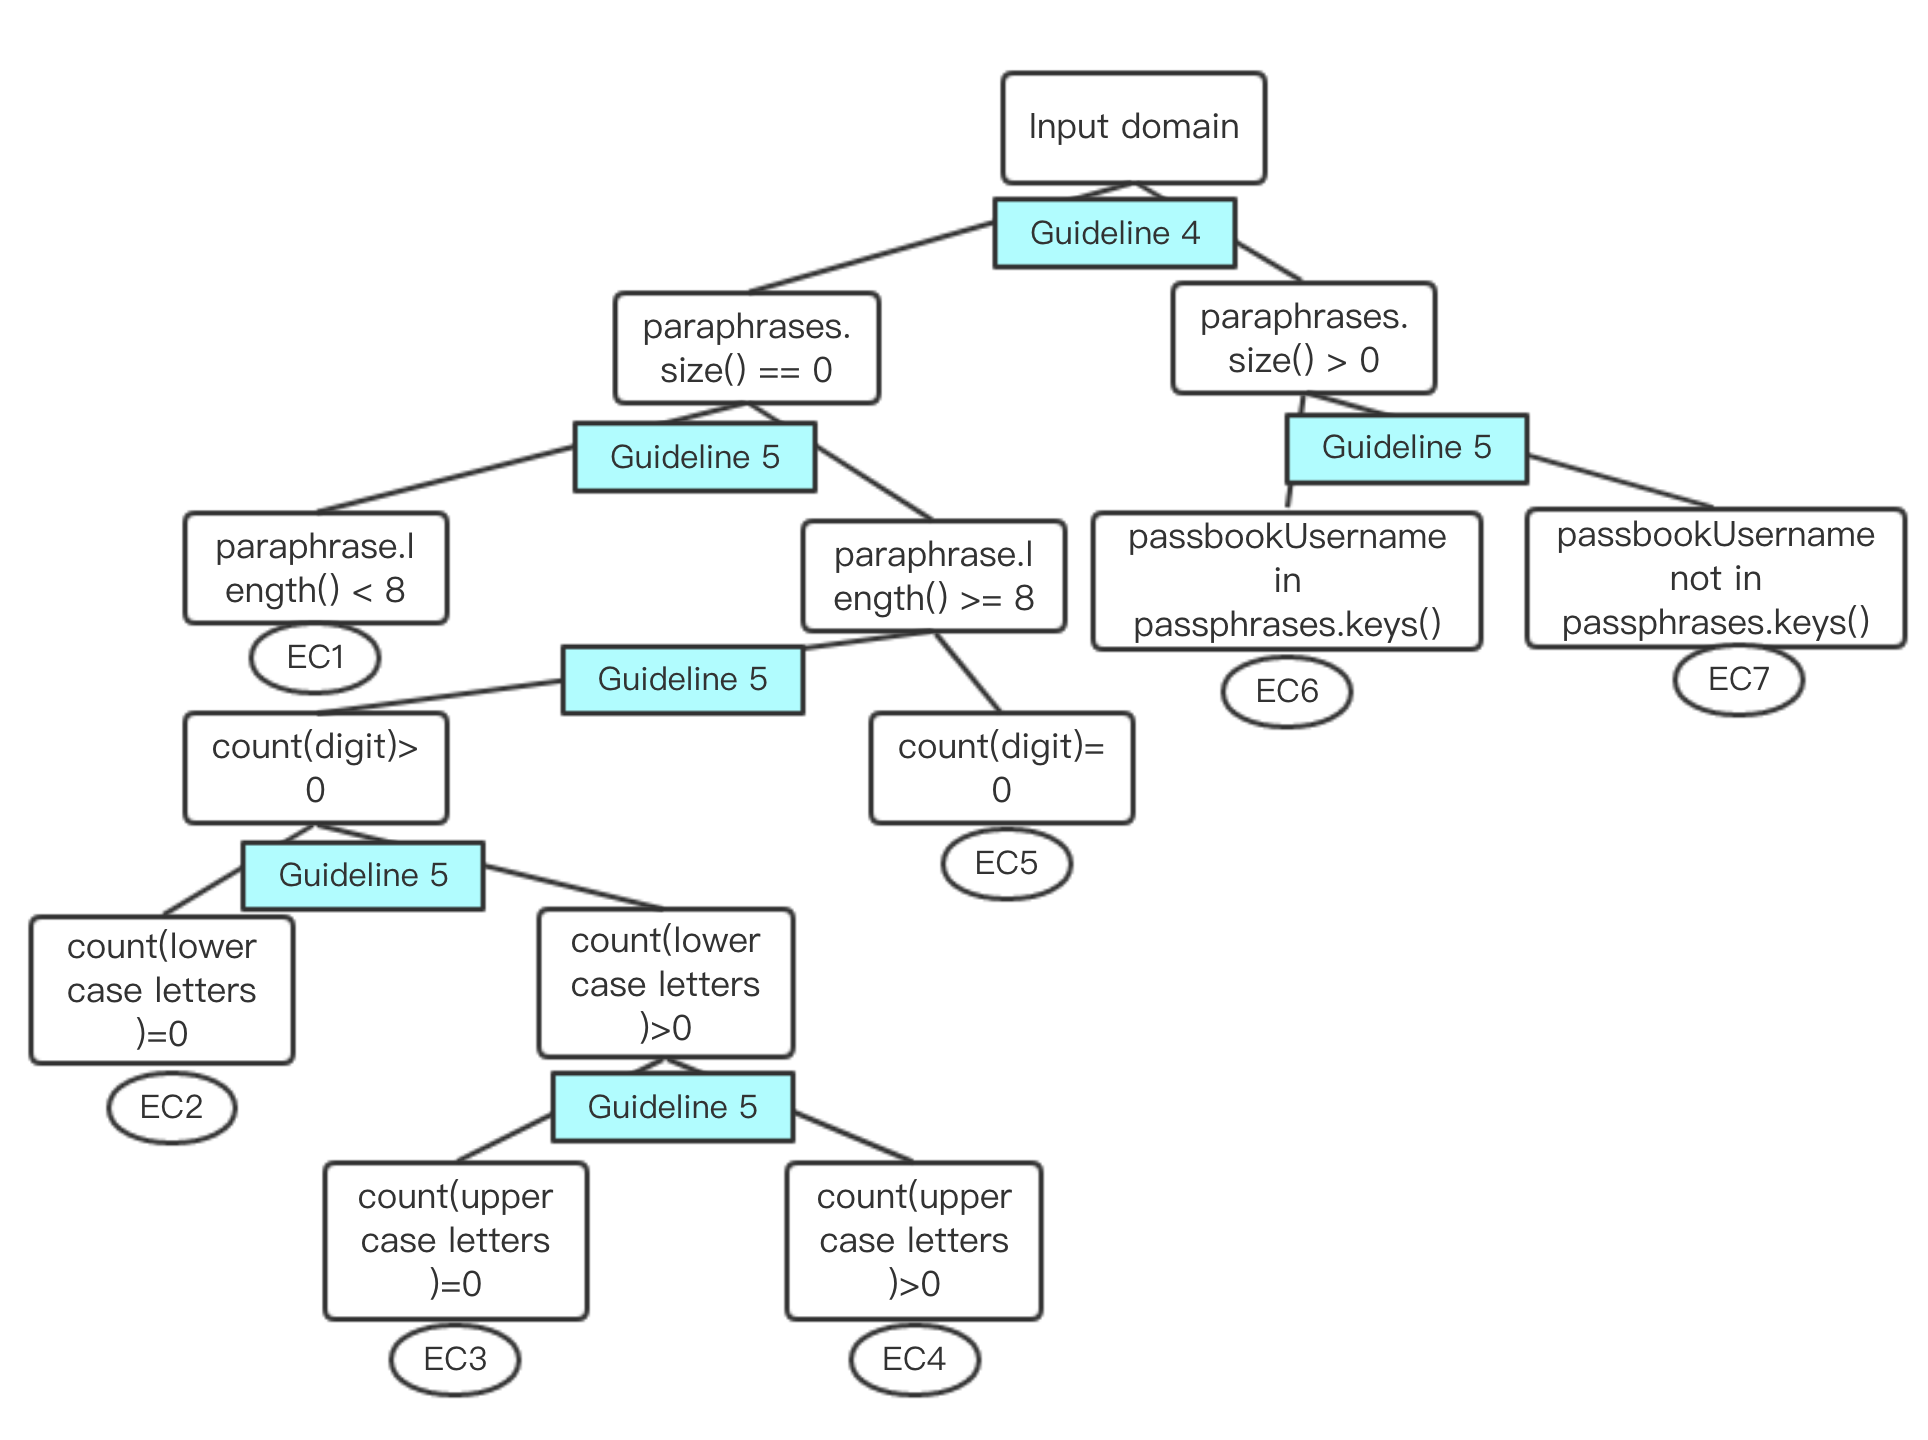
\includegraphics[width=17cm]  {addUserNew.png}}        
\caption{\label{1} Test template tree for addUser()}      
\end{figure}
\begin{figure}[hbt!]        
\center{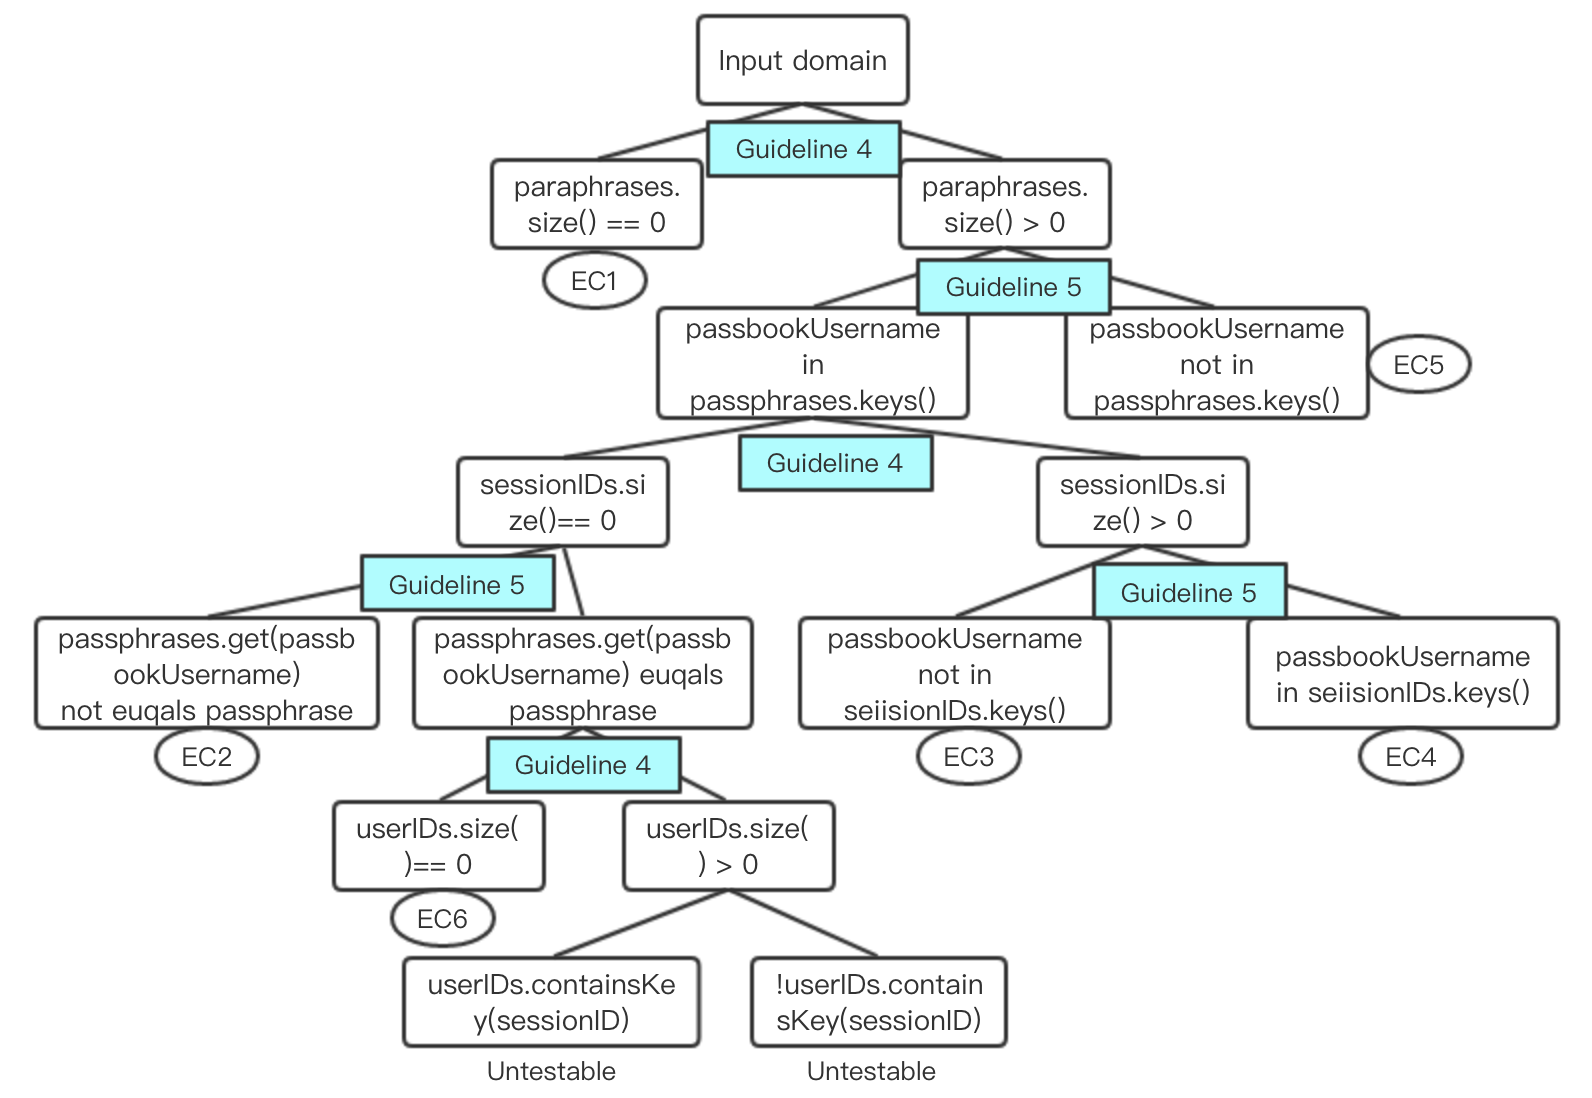
\includegraphics[width=15cm]  {loginUserNew.png}}        
\caption{\label{1} Test template tree for loginUser()}      
\end{figure}
\begin{figure}[hbt!]        
\center{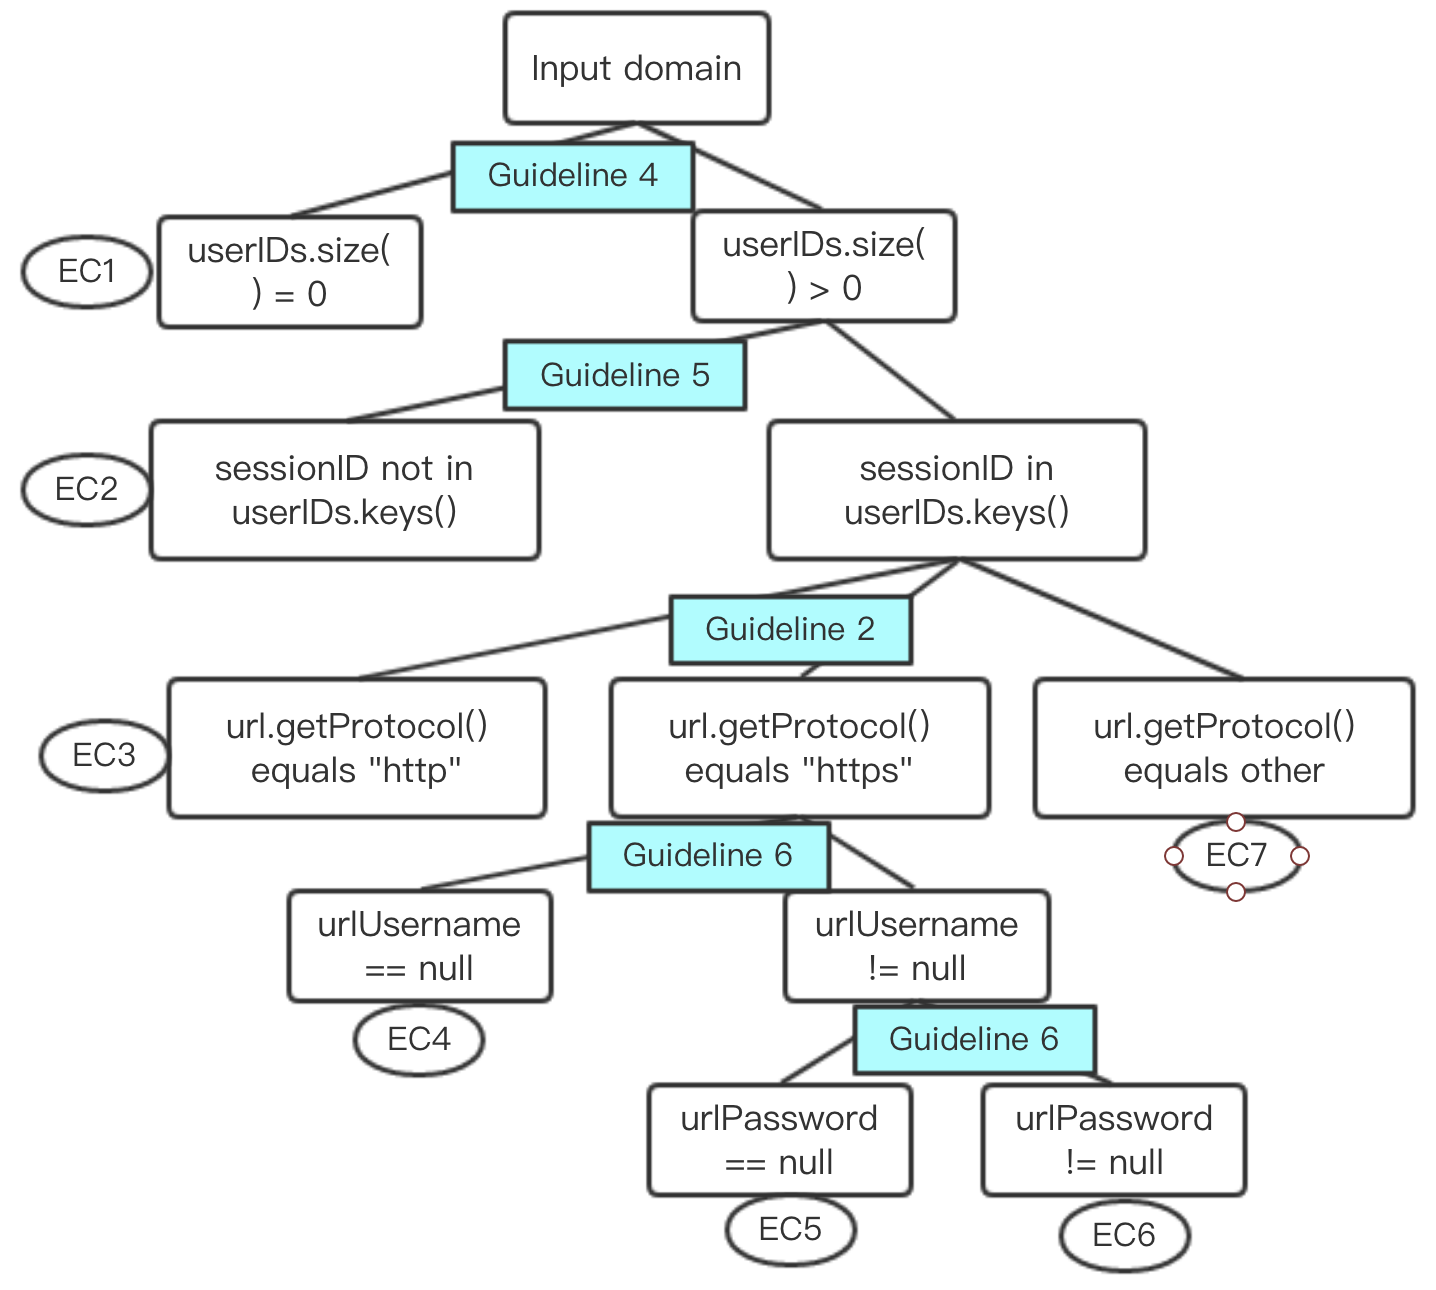
\includegraphics[width=11cm]  {updateDetailsNew.png}}        
\caption{\label{1} Test template tree for updateDetails()}      
\end{figure}
\begin{figure}[t!]        
\center{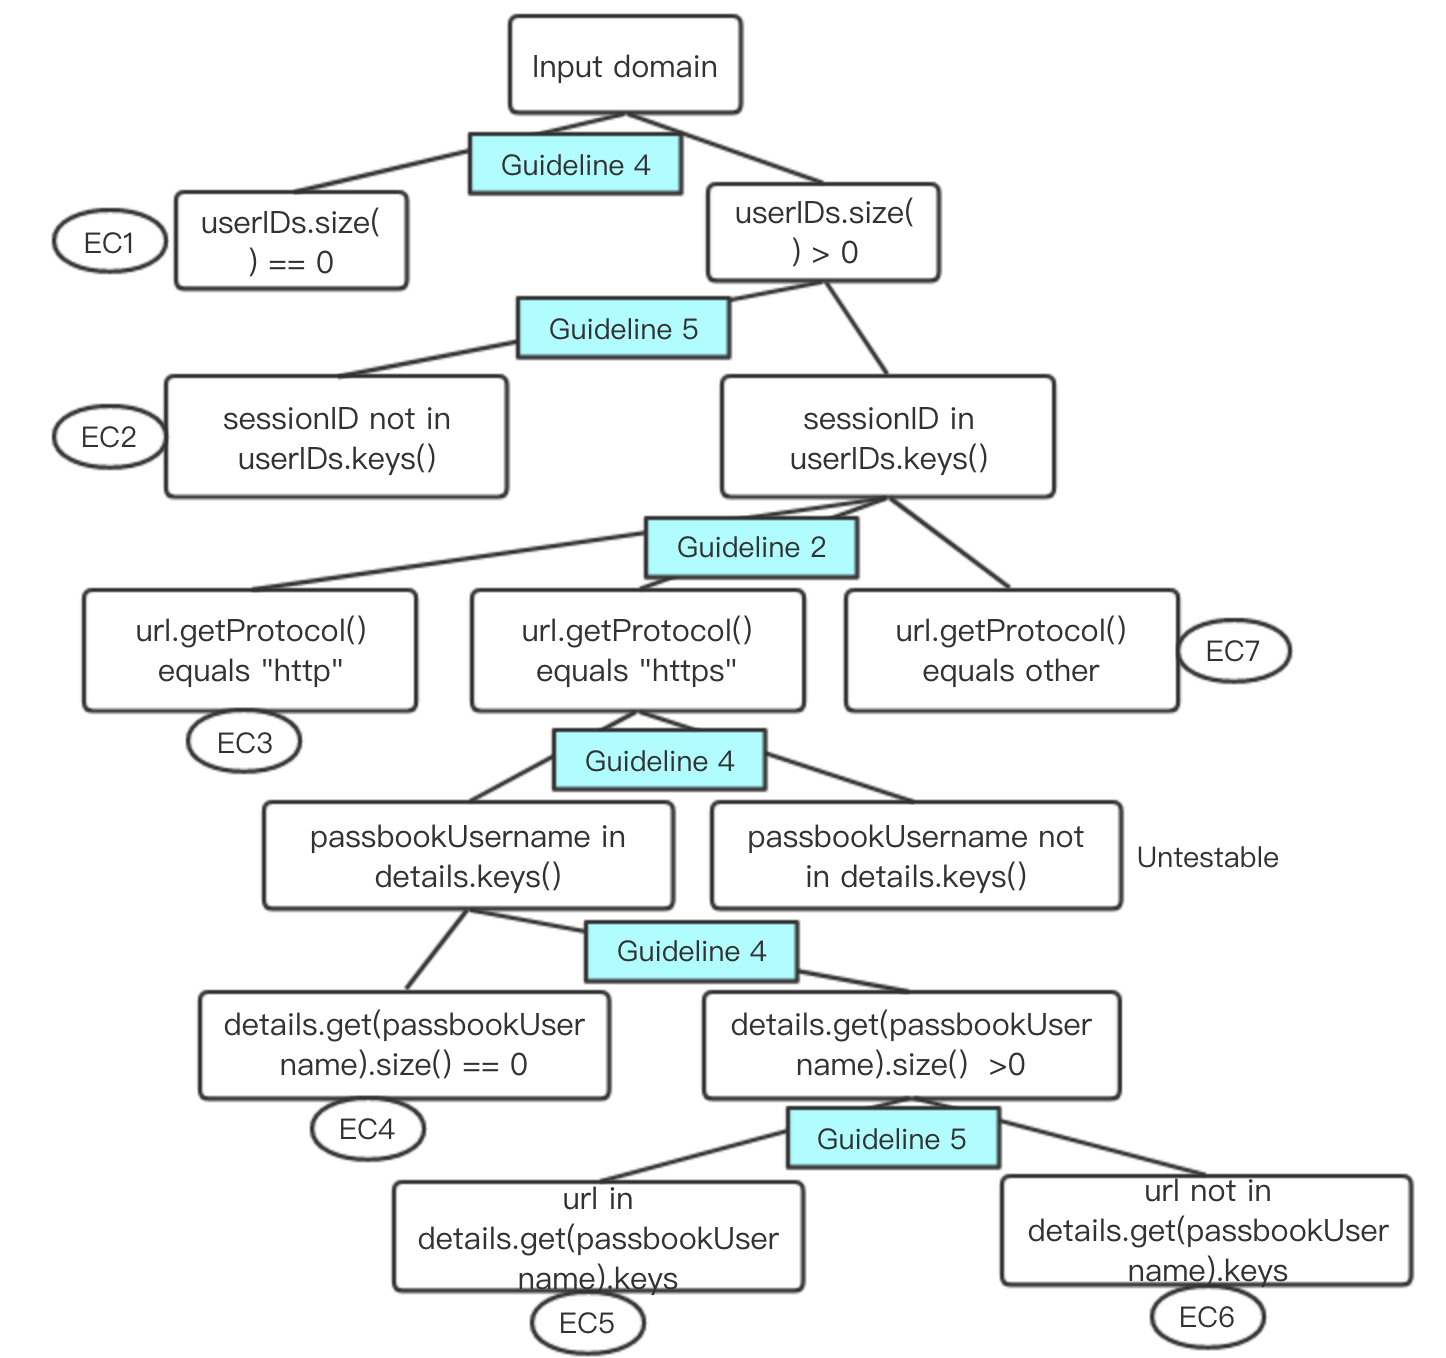
\includegraphics[width=12cm]  {retrieveDetailsNew.png}}        
\caption{\label{1} Test template tree for retrieveDetails()}      
\end{figure}

\subsection{Do your set of equivalence classes cover the input space?}
My set of equivalence classes cover the input space. The reasons are as follows:
\begin{itemize}
\item [1)] All leaf nodes are divided strictly and carefully, so that they do not overlap with other leaf.
\item [2)] The collection of the set of each sibling node covers all the cases of their parent node.
\item [3)]
If two variables are independent of each other, then the subtree of one variable can be added to a leaf node of the other variable. In this case, all the nodes add up to cover all situations.
\item [4)]
As part of your input domain, the instance variables should also be considered. Note that all of these variables are collections, so according to guideline 4, we should follow the zero-one-many rule. But in this particular case, we just care about whether the collection contains some values. So I combined the two cases (number of elements equals 1 and greater than 1) into one (greater than 0), which does not affect the results of the tests.
\end{itemize}

\section{Test cases associated with equivalence classes}
\subsection{addUser}

\begin{longtable}{|p{2cm}|p{7cm}|p{5cm}|}
\caption{Test cases for addUser}\\
\hline 
ID&Test case&Expected output\\
\hline  
EC1&paraphrases = \{\}, passbookUsername = "abc", paraphrase = "12345aA"&WeakPassphraseException\\
\hline
EC2&paraphrases = \{\}, passbookUsername = "abc", paraphrase = "1234567A"&WeakPassphraseException\\
\hline
EC3&paraphrases = \{\}, passbookUsername = "abc", paraphrase = "1234567a"&WeakPassphraseException\\
\hline
EC4&paraphrases = \{\}, passbookUsername = "abc", paraphrase = "123456aA"&-\\
\hline
EC5&paraphrases = \{\}, passbookUsername = "abc", paraphrase = "abcdABCD"&WeakPassphraseException\\
\hline
EC6&paraphrases = \{"abcd":"123456aA"\}, passbookUsername = "abcd", paraphrase = "123456aA"&DuplicateUserException\\
\hline
EC7&paraphrases = \{"abcd":"123456aA"\}, passbookUsername = "abc", paraphrase = "123456aA"&-\\
\hline
\end{longtable}

\subsection{loginUser}

\begin{longtable}{|p{2cm}|p{7cm}|p{5cm}|}
\caption{Test cases for loginUser}\\
\hline 
ID&Test case&Expected output\\
\hline  
EC1&paraphrases = \{\}, sessionIDs = \{\}, userIDs = \{\}, passbookUsername = "abc", paraphrase = "123456aA"&NoSuchUserException\\
\hline
EC2&paraphrases = \{"abc":"123456aA"\}, sessionIDs = \{\}, userIDs = \{\} passbookUsername = "abc", paraphrase = "123456aB"&IncorrectPassphraseException\\
\hline
EC3&paraphrases = \{"abc":"123456aA"\}, sessionIDs = \{\}, userIDs = \{\} passbookUsername = "abc", paraphrase = "123456aA"&...\\
\hline
EC4&paraphrases = \{"abc":"123456aA"\}, sessionIDs = \{\}, userIDs = \{123:"def"\} passbookUsername = "abc", paraphrase = "123456aA"&...\\
\hline
EC5&paraphrases = \{"abc":"123456aA"\}, sessionIDs = \{"def":123\}, userIDs = \{\} passbookUsername = "abc", paraphrase = "123456aA"&...\\
\hline
EC6&paraphrases = \{"abc":"123456aA"\}, sessionIDs = \{"abc":123\}, userIDs = \{\} passbookUsername = "abc", paraphrase = "123456aA"&AlreadyLoggedInException\\
\hline
EC7&paraphrases = \{"abc":"123456aA"\}, sessionIDs = \{\}, userIDs = \{\} passbookUsername = "abcd", paraphrase = "123456aA"&NoSuchUserException\\
\hline
\end{longtable}


\subsection{updateDetails}
\begin{longtable}{|p{2cm}|p{7cm}|p{5cm}|}
\caption{Test cases for updateUserDetails}\\
\hline 
ID&Test case&Expected output\\
\hline  
EC1&userIDs = \{\}, sessionID = 123, url = "http://test.com", urlUsername = "123", urlPassword = "123"&InvalidSessionIDException\\
\hline
EC2&userIDs = \{123:"abc"\}, sessionID = 456, url = "http://test.com", urlUsername = "123", urlPassword = "123"&InvalidSessionIDException\\
\hline
EC3&userIDs = \{123:"abc"\}, sessionID = 123, url = "http://test.com", urlUsername = "123", urlPassword = "123"&-\\
\hline
EC4&userIDs = \{123:"abc"\}, sessionID = 123, url = "https://test.com", urlUsername = null, urlPassword = null&-\\
\hline
EC5&userIDs = \{123:"abc"\}, sessionID = 123, url = "https://test.com", urlUsername = null, urlPassword = "123"&-\\
\hline
EC6&userIDs = \{123:"abc"\}, sessionID = 123, url = "https://test.com", urlUsername = "123", urlPassword = null&-\\
\hline
EC7&userIDs = \{123:"abc"\}, sessionID = 123, url = "https://test.com", urlUsername = "123", urlPassword = "123"&-\\
\hline
EC8&userIDs = \{123:"abc"\}, sessionID = 123, url = "ftp://test.com", urlUsername = "123", urlPassword = "123"&MalformedURLException\\
\hline
\end{longtable}
\subsection{retrieveDetails}
%TODO

%---------------------------------------------------------------------------------------
\section{Boundary-value analysis}
\subsection{addUser}

\begin{longtable}{|p{0.5cm}|p{0.5cm}|p{7cm}|p{5cm}|}
\caption{Test cases for addUser}\\
\hline 
Test ID&EC&Test case&Boundary\\
\hline  
1&EC1&paraphrases = \{\}, passbookUsername = "abc", paraphrase = "12345aA"&off point for paraphrase.length() < 8\\
\hline
2&EC2&paraphrases = \{\}, passbookUsername = "abc", paraphrase = "123456`A"&off point for S[i] not in ‘a’ - ‘z’, for every 0 <= i <= length[paraphrase]-1\\
\hline
3&EC2&paraphrases = \{\}, passbookUsername = "abc", paraphrase = "123456\{A"&off point for S[i] not  in ‘a’ - ‘z’, for every 0 <= i <= length[paraphrase]-1\\
\hline
4&EC3&paraphrases = \{\}, passbookUsername = "abc", paraphrase = "123456@a"&off point for S[i] not in ‘A’ - ‘Z’, for every 0 <= i <= length[paraphrase]-1\\
\hline
5&EC3&paraphrases = \{\}, passbookUsername = "abc", paraphrase = "123456[a"&off point for S[i] not  in ‘A’ - ‘Z’, for every 0 <= i <= length[paraphrase]-1\\
\hline
6&EC4&paraphrases = \{\}, passbookUsername = "abc", paraphrase = "234567nA"&on point for S[i] in ‘A’ - ‘Z’, for some 0 <= i <= length[paraphrase]-1\\
\hline
7&EC4&paraphrases = \{\}, passbookUsername = "abc", paraphrase = "234567nZ"&on point for S[i] in ‘A’ - ‘Z’, for some 0 <= i <= length[paraphrase]-1\\
\hline
8&EC4&paraphrases = \{\}, passbookUsername = "abc", paraphrase = "234567Na"&on point for S[i] in ‘a’ - ‘z’, for some 0 <= i <= length[paraphrase]-1\\
\hline
9&EC4&paraphrases = \{\}, passbookUsername = "abc", paraphrase = "234567Nz"&on point for S[i] in ‘a’ - ‘z’, for some 0 <= i <= length[paraphrase]-1\\
\hline
10&EC4&paraphrases = \{\}, passbookUsername = "abc", paraphrase = "abcdABC0"&on point for S[i] in ‘0’ - ‘9’, for some 0 <= i <= length[paraphrase]-1\\
\hline
11&EC4&paraphrases = \{\}, passbookUsername = "abc", paraphrase = "abcdABC9"&on point for S[i] in ‘0’ - ‘9’, for some 0 <= i <= length[paraphrase]-1\\
\hline
12&EC5&paraphrases = \{\}, passbookUsername = "abc", paraphrase = "abcdABC/"&off point for S[i] not in ‘0’ - ‘9’, for every 0 <= i <= length[paraphrase]-1\\
\hline
13&EC5&paraphrases = \{\}, passbookUsername = "abc", paraphrase = "abcdABC:"&off point for S[i] not in ‘0’ - ‘9’, for every 0 <= i <= length[paraphrase]-1\\
\hline
14&EC6&paraphrases = \{"abcd":"123456aA"\}, passbookUsername = "abcd", paraphrase = "123456aA"&on point for passbookUsername in passphrases.keys()\\
\hline
15&EC7&paraphrases = \{"abcd":"123456aA"\}, passbookUsername = "abc", paraphrase = "123456aA"&on point for passbookUsername not in passphrases.keys()\\
\hline
\end{longtable}

\subsection{loginUser}

\begin{longtable}{|p{0.5cm}|p{0.5cm}|p{7cm}|p{5cm}|}
\caption{Test cases for loginUser}\\
\hline 
Test ID&EC&Test case&Boundary\\
\hline  
1&EC1&paraphrases = \{\}, sessionIDs = \{\}, userIDs = \{\}, passbookUsername = "abc", paraphrase = "123456aA"&on point for paraphrases.size() == 0\\
\hline
2&EC2&paraphrases = \{"abc":"123456aA"\}, sessionIDs = \{\}, userIDs = \{\} passbookUsername = "abc", paraphrase = "123456aB"&on point for passphrases.get (passbookUsername)
not euqals passphrase\\
\hline
3&EC3&paraphrases = \{"abc":"123456aA"\}, sessionIDs = \{\}, userIDs = \{\} passbookUsername = "abc", paraphrase = "123456aA"&on point for userIDs.size()== 0\\
\hline
4&EC4&paraphrases = \{"abc":"123456aA"\}, sessionIDs = \{\}, userIDs = \{123:"def"\} passbookUsername = "abc", paraphrase = "123456aA"&off point for userIDs.size() > 0 and paraphrases.size() > 0\\
\hline
5&EC5&paraphrases = \{"abc":"123456aA"\}, sessionIDs = \{"def":123\}, userIDs = \{\} passbookUsername = "abc", paraphrase = "123456aA"&on point for passbookUsername not in sessionIDs.keys() and off point for sessionIDs.size() > 0\\
\hline
6&EC6&paraphrases = \{"abc":"123456aA"\}, sessionIDs = \{"abc":123\}, userIDs = \{\} passbookUsername = "abc", paraphrase = "123456aA"&on point for passbookUsername in sessionIDs.keys()\\
\hline
7&EC7&paraphrases = \{"abc":"123456aA"\}, sessionIDs = \{\}, userIDs = \{\} passbookUsername = "abcd", paraphrase = "123456aA"&on point for passbookUsername not in passphrases.keys()\\
\hline
\end{longtable}

\subsection{updateDetails}
\begin{longtable}{|p{0.5cm}|p{0.5cm}|p{7cm}|p{5cm}|}
\caption{Test cases for updateUserDetails}\\
\hline 
Test ID&EC&Test case&Boundary\\
\hline  
1&EC1&userIDs = \{\}, sessionID = 123, url = "http://test.com", urlUsername = "123", urlPassword = "123"&on point for userIDs.size() == 0\\
\hline
2&EC2&userIDs = \{123:"abc"\}, sessionID = 456, url = "http://test.com", urlUsername = "123", urlPassword = "123"&on point for sessionID not in userIDs.keys() and off point for userIDs.size() > 0\\
\hline
3&EC3&userIDs = \{123:"abc"\}, sessionID = 123, url = "http://test.com", urlUsername = "123", urlPassword = "123"&on point for url.getProtocol() equals "http"\\
\hline
4&EC4&userIDs = \{123:"abc"\}, sessionID = 123, url = "https://test.com", urlUsername = null, urlPassword = null&on point for urlUsername == null and urlPassword == null and url.getProtocol() equals "https"\\
\hline
5&EC5&userIDs = \{123:"abc"\}, sessionID = 123, url = "https://test.com", urlUsername = null, urlPassword = "123"&on point for urlUsername == null and urlPassword != null\\
\hline
6&EC6&userIDs = \{123:"abc"\}, sessionID = 123, url = "https://test.com", urlUsername = "123", urlPassword = null&on point for urlUsername != null and urlPassword == null\\
\hline
7&EC7&userIDs = \{123:"abc"\}, sessionID = 123, url = "https://test.com", urlUsername = "123", urlPassword = "123"&on point for urlUsername != null and urlPassword != null\\
\hline
8&EC8&userIDs = \{123:"abc"\}, sessionID = 123, url = "ftp://test.com", urlUsername = "123", urlPassword = "123"&off point for url.getProtocol() equals other\\
\hline
\end{longtable}
\subsection{retrieveDetails}
%TODO


%---------------------------------------------------------------------------------------
\section{Multiple-conditions coverage}
\subsection{addUser}
\begin{longtable}{|p{2cm}|p{10cm}|p{3cm}|}
\caption{Multiple-conditions for addUser}\\
\hline 
Test Objective ID&Condition&Output(s)\\
\hline  
1&passphrases.containsKey(passbookUsername)&true\\
\hline
2&passphrases.containsKey(passbookUsername)&false\\
\hline
3&passphrase.length() \textless MINIMUM\_PASSPHRASE\_LENGTH&true\\
\hline
4&passphrase.length() \textless MINIMUM\_PASSPHRASE\_LENGTH&false\\
\hline
5&i < passphrase.length()&true\\
\hline
6&i < passphrase.length()&false\\
\hline
7&'a' <= passphrase.charAt(i) \&\& passphrase.charAt(i) <= 'z'&false false\\
\hline
8&'a' <= passphrase.charAt(i) \&\& passphrase.charAt(i) <= 'z'&true false\\
\hline
9&'a' <= passphrase.charAt(i) \&\& passphrase.charAt(i) <= 'z'&false true\\
\hline
10&'a' <= passphrase.charAt(i) \&\& passphrase.charAt(i) <= 'z'&true true\\
\hline
11&'A' <= passphrase.charAt(i) \&\& passphrase.charAt(i) <= 'Z'&false false\\
\hline
12&'A' <= passphrase.charAt(i) \&\& passphrase.charAt(i) <= 'Z'&true false\\
\hline
13&'A' <= passphrase.charAt(i) \&\& passphrase.charAt(i) <= 'Z'&false true\\
\hline
14&'A' <= passphrase.charAt(i) \&\& passphrase.charAt(i) <= 'Z'&true true\\
\hline
15&'0' <= passphrase.charAt(i) \&\& passphrase.charAt(i) <= '9'&false false\\
\hline
16&'0' <= passphrase.charAt(i) \&\& passphrase.charAt(i) <= '9'&true false\\
\hline
17&'0' <= passphrase.charAt(i) \&\& passphrase.charAt(i) <= '9'&false true\\
\hline
18&'0' <= passphrase.charAt(i) \&\& passphrase.charAt(i) <= '9'&true true\\
\hline
19&!containsLowerCase || !containsUpperCase || !containsNumber&false false false\\
\hline
20&!containsLowerCase || !containsUpperCase || !containsNumber&false false true\\
\hline
21&!containsLowerCase || !containsUpperCase || !containsNumber&false true false\\
\hline
22&!containsLowerCase || !containsUpperCase || !containsNumber&false true true\\
\hline
23&!containsLowerCase || !containsUpperCase || !containsNumber&true false false\\
\hline
24&!containsLowerCase || !containsUpperCase || !containsNumber&true false true\\
\hline
25&!containsLowerCase || !containsUpperCase || !containsNumber&true true false\\
\hline
26&!containsLowerCase || !containsUpperCase || !containsNumber&true true true\\
\hline
\end{longtable}

\subsection{loginUser}
\begin{longtable}{|p{2cm}|p{10cm}|p{3cm}|}
\caption{Multiple-conditions for loginUser}\\
\hline 
Test Objective ID&Condition&Output(s)\\
\hline  
1&!passphrases.containsKey(passbookUsername)&true\\
\hline
2&!passphrases.containsKey(passbookUsername)&false\\
\hline
3&sessionIDs.get(passbookUsername) != null&true\\
\hline
4&sessionIDs.get(passbookUsername) != null&false\\
\hline
5&!passphrases.get(passbookUsername).equals(passphrase)&true\\
\hline
6&!passphrases.get(passbookUsername).equals(passphrase)&false\\
\hline
7&userIDs.containsKey(sessionID)&true\\
\hline
8&userIDs.containsKey(sessionID)&false\\
\hline
\end{longtable}

\subsection{updateDetails}
\begin{longtable}{|p{2cm}|p{11cm}|p{2cm}|}
\caption{Multiple-conditions for updateDetails}\\
\hline 
Test Objective ID&Condition&Output(s)\\
\hline  
1&passbookUsername == null&true\\
\hline
2&passbookUsername == null&false\\
\hline
3&!Arrays.asList(VALID\_URL\_PROTOCOLS).contains(url.getProtocol())&true\\
\hline
4&!Arrays.asList(VALID\_URL\_PROTOCOLS).contains(url.getProtocol())&false\\
\hline
5&urlUsername == null || urlPassword == null&false false\\
\hline
6&urlUsername == null || urlPassword == null&false true\\
\hline
7&urlUsername == null || urlPassword == null&true false\\
\hline
8&urlUsername == null || urlPassword == null&true true\\
\hline
\end{longtable}

\subsection{retrieveDetails}
\begin{longtable}{|p{2cm}|p{11cm}|p{2cm}|}
\caption{Multiple-conditions for retrieveDetails}\\
\hline 
Test Objective ID&Condition&Output(s)\\
\hline  
1&passbookUsername == null&true\\
\hline
2&passbookUsername == null&false\\
\hline
3&!Arrays.asList(VALID\_URL\_PROTOCOLS).contains(url.getProtocol())&true\\
\hline
4&!Arrays.asList(VALID\_URL\_PROTOCOLS).contains(url.getProtocol())&false\\
\hline
5&pt == null&false\\
\hline
6&pt == null&true\\
\hline
7&pair == null&false\\
\hline
8&pair == null&true\\
\hline
\end{longtable}

\enddocument